\documentclass[a4paper, 12pt]{article}
\usepackage[utf8]{inputenc}
\usepackage{geometry}
\usepackage{polski}
\usepackage{graphicx}
\usepackage{float}
\usepackage{etoolbox,refcount}
\usepackage{multicol}

\newgeometry{left=2cm, right=2cm, bottom=2cm, top=1.5cm}

\begin{document}
	\begin{figure}[H]
		\centering
		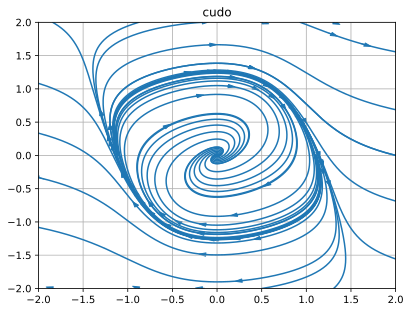
\includegraphics[width = \textwidth]{./img/cudo.png}
	\end{figure}
	\section{Cel ćwiczenia}
		Celem ćwiczenia jest zapoznanie się z zasadami programowania sterowników PLC z wykorzystaniem języka schematów drabinkowych LD -- jednego ze standardowych narzędzi programowania sterowników PLC.
	\section{Schemat stanowiska}
		Stanowisko składa się z dwóch części: 
		\begin{itemize}
			\item[--] regulator z panelem operatorskim i osprzętem dodatkowym -- zespół przełączników cyfrowych, gniazdo wyjść cyfrowych i zespół gniazd dla wejść, gdzie do jednego jest podłączony zasilacz z regulowanym napięciem/prądem i wyjść analogowych, gdzie do jednego jest podłączony woltomierz
			\item[--] komputer klasy PC z oprogramowaniem RSLOGI500 STARTER umożliwiającym programowanie sterownika, połączony ze sterownikiem przez łącze szeregowe RS232
		\end{itemize}
		\begin{figure}[H]
			\centering
			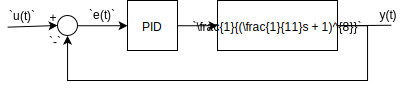
\includegraphics[height=6cm, width=\textwidth]{./img/schemat.png}
			\caption{Uproszczony schemat układu}
		\end{figure}
	\section{Wstęp}
		Sterowniki PLC są chętnie wykorzystywane w przemyśle ze względu na swoją uniwersalność, prostotę oraz niezawodność. Są to układy sekwencyjnymi działającymi na mikroprocesorach, służące do sterowania pracą urządzenia technologicznego. Aby jednak poprawnie działać sterownik PLC potrzebuje wgranego algorytmu dopasowanego do wymaganego zastosowania. Sterownik PLC posiada cykliczny obieg pamięci programu - po zakończeniu działania algorytmu jest on przeprowadzany od nowa.
		\newline
		\newline
		\noindent Metody programowania sterowników PLC są unormowane. Do tych metod należą schematy drabinkowe LD, które są graficznym, logicznym, prostym i przejrzystym językiem programowania. Wiele środowisk programistycznych pozwala na podglądanie wykonywania się programów jako przesył sygnału na schemacie drabinkowym na podłączonym do sterownika, co samo\linebreak w sobie stanowi graficzny interfejs użytkownika.
		\newline
		\newline 
		Język drabinkowy składa się z funkcji, bloków funkcyjnych, cewek oraz styków. Funkcja jest tu zdefiniowana tak jak funkcja matematyczna -- dla danego zestawu argumentów wejściowych zawsze poda ten sam wynik. Blok funkcyjny może dawać różne wyniki dla tych samych wejść w zależności od swojego stanu -- zachowuje się jak automat. Cewki przepuszczają sygnał i zapisują go w pewien charakterystyczny dla swojego typu sposób pod pewnym adresem, a styki przepuszczają sygnał zależnie od zachowania wartości pod adresem, który jest do nich przypisany.
	\section{Przeprowadzenie ćwiczenia}
		Ćwiczenie rozpoczęliśmy od konfiguracji środowiska programistycznego i ustalenia komunikacji między komputerem, a sterownikiem. Po wstępnym zapoznaniu się ze środowiskiem pracy przystąpiliśmy do wykonywania kolejnych poleceń z instrukcji.
		\subsection{Regulator dwupołożeniowy}
			Regulator dwupołożeniowy działa na zasadzie podawania sygnału wysokiego na wyjście dyskretne w sytuacji kiedy wartość na wejściu będzie niższa od wartości referencyjnej podanej przez nas w trakcie projektowania programu na wyjściu powinien pojawić się sygnał wysoki.
			\begin{figure}[H]
				\centering
				\includegraphics[width=0.8\textwidth]{./img/dwa_pol.png}
				\caption{Regulator dwupołożeniowy}
			\end{figure}
			\noindent Program korzysta z wejścia analogowego AI 01, gdyż tam jest podłączony generator i z wyjścia dyskretnego DO 01 -- kontrolka na kontrolerze. 
		\subsection{Regulator P}
			Regulator P pobiera na wejściu pewnien sygnał analogowy, a następnie zależnie od ustawienia na wzmocnienie równe 0.5 lub wzmocnienie równe 0.25 sygnał wejściowy jest przepuszczany przez bloczek dzielący go przez 2 lub przez 4, zależnie od wybranego zastosowania. Na schemacie zamieszczonym tu dzielenie następuje przez 2. Na wejściu układu dzielącego znajduje się różnica między wartością zadaną, a wartością podaną na wejściu analogowym
			\begin{figure}[H]
				\centering
				\includegraphics[width=0.8\textwidth]{./img/prop.png}
				\caption{Regulator proporcjonalny}
			\end{figure}
		\noindent Zachowanie układu dla obydwu wzmocnień obserwowaliśmy na woltomierzu, który był podłączony do wyjścia analogowego.
		\subsection{Generator sygnału prostokątnego o okresie 10 s}
			Generator sygnału prostokątnego miał być wykonany z dwóch timerów TON oraz ze styków normalnie zamkniętych. Dodatkowo układ miał być uruchamiany wyjściem analogowym DI 01, a na celu miał przełączanie wyjścia dyskretnego DO 00 co 10 sekund.
			\begin{figure}[H]
				\centering
				\includegraphics[width=0.8\textwidth]{./img/timer.png}
				\caption{Generator sygnału prostokątnego}
			\end{figure}
	\section{Wnioski}
		Ćwiczenie zostało zakończone pomyślnie, wszystkie jego cele zostały zrealizowane bez większych problemów i komplikacji. Regulator dwupołożeniowy, regulator P oraz generator fali prostokątnej działa zgodnie ze specyfikacją podaną w instrukcji do zadania.
		\newline
		\newline
		Kilka podejść opartych na metodzie prób i błędów zaznajomiło nas z nazewnictwem funkcji środowiska programistycznego z jakim mieliśmy do czynienia -- wszystkie polecenia jakie były tam wykonywane były poleceniami dawanymi ,,z pozycji sterownika''. Przykładem tego są polecenia DOWNLOAD/UPLOAD, które pozwalały odpowiednio na zgranie programu z komputera na sterownik oraz pobranie ze sterownika programu na komputer, a nie pobranie na komputer programu ze sterownika i wgranie programu na sterownik. Na szczęście udało się szybko zauważyć ten problem i przystąpić do kontynuacji ćwiczenia.
		\newline
		\newline
		Nauczyliśmy się kolejnego systemu adresowania na sterownika PLC, który był inny niż ten z którym się zetknęliśmy wykonując laboratorium nr 3. Dowiedzieliśmy się tym samym, że nie jest to pewien standard uniwersalny dla wszystkich sterowników klasy PLC.
		\newline
		\newline 
		Ćwiczenie to pozwoliło nam na zapoznanie się z timerami oraz z zasadami budowania układów związanych z nimi. Jest to wiedza uniwersalna, wykraczająca swoim zastosowaniem poza programowanie sterowników PLC. Timery występują chociażby w programowaniu układów FPGA, które nie są układami sekwencyjnymi tak jak sterowniki PLC. 
		\newline
		\newline
		Możliwość podglądu wykonywania się programu pozwoliła nam na szybkie korekty błędów, jakie powstawały w trakcie tworzenia programu. Jest to efektywna metoda debugowania, która z powodzeniem znalazła zastosowanie w wielu innych graficznych językach programowania takich jak np. LabVIEW.
		\newline 
		\newline
		Po raz trzeci w toku edukacji mieliśmy styczność ze sterownikiem PLC i programowaliśmy w języku drabinkowym, zdobywając w tym coraz większą wprawę i zaznajamiając się z różnorodnością środowisk programistycznych języka drabinkowego. Jak do tej pory jest to najstarsza forma oprogramowania z jaką mieliśmy styczność, jednak w praktyce zawodowej nie zawsze ma się wygodę wyboru środowiska programistycznego ze względu na dużą trwałość tych sterowników i brak konieczności ich wymiany.
\end{document}
